\documentclass{article}
\usepackage[utf8]{inputenc}

\title{TT3010 - Audio technology and room acoustics. \newline Exercise 3 - Loudspeakers.}


%\author{Jan Arne Bosnes}
\date{\today}

\usepackage{natbib}
\usepackage{graphicx}
\usepackage{multicol}
\usepackage{gensymb}
\usepackage{float}


\begin{document}

\maketitle

All tasks are based on chapter 19 in "Science of Sound". It is recommended that the student will try to do every task, but tasks marked \textit{Mandatory} are to be handed in for approval (online). The deadline is specified in blackboard.

\section*{Tasks}
%\begin{multicols}{2}
\begin{itemize}
    \item [1.] \textit{Mandatory.} Compare the sound power level of a loudspeaker with an efficiency of 1 \% to one with an efficiency of 10 \% supplied with the same electrical power (the difference should be expressed in dB).
        
    \item[2.] Compare the cone areas of speakers having diameters of 20 cm, 30 cm and 38 cm (8 in., 12 in., and 15 in.).  
        
    \item[3.] A loudspeaker 20 cm in diameter is mounted at the center of a 1-m square baffle board.
    
    \begin{itemize}
        \item [a.] Determine the path length from the center of the front side to the center of the back side of the speaker.
        \item [b.] At which frequency will this path be equal to one-half wavelength of sound?
    \end{itemize}
    
    \item[4.] \textit{Mandatory.}
    \begin{itemize}
        \item [a.] From the graph shown in figure \ref{fig:abs}, determine the volume of air that must be moved in order to generate a sound power of 0.1 W at 100 Hz.
        \item [b.] How far must a speaker cone move in order to move this volume of air if the cone has a diameter of 20 cm?
    \end{itemize}
    
    %\item[5.] \textit{Not relevant for this course} For satisfactory operation down to a cutoff frequency $f_c$, a horn loudspeaker should have a mouth diameter at least one-fourth of the wavelength at $f_c$, and its diameter should double no more rapidly than every one-ninth of the wavelength at $f_c$. Determine the mouth diameter and the total length of a horn loudspeaker with $f_c=100 Hz$ if the throat diameter is 5.4 cm.   
        
    \item[5.] \textit{Mandatory} If a loudspeaker can produce a sound pressure level of 92 dB for 1 W of input power at a distance of 1 m, estimate its efficiency, in $\%$, in converting electrical power to acoustical power. (Hint: Assume that the sound is uniformly radiated into a hemisphere so that the sound pressure level, $L_p = SPL$, at 1 m is 8 dB less than the sound power level, $L_W$.)

    
    \item[6.] How large a volume of air must be moved by a loudspeaker cone radiating 0.1 W of acoustical power at 50 Hz? How far would the cone of a 30 cm loudspeaker (actual cone diameter is 25 cm) have to move to displace this volume?
    
    \item[7.] \textit{Mandatory.} A certain loudspeaker has a compliance of 8.7 $\cdot 10^{-4}$ m/N and a mass (cone plus voice coil) of 71 g. Estimate its resonance frequency. (The compliance is the reciprocal of the stiffness or spring constant: $C=1/K$).
    
    %\item[9.] \textit{Not relevant for this course} Express the compliance of the loudspeaker in task 8 in cm/dyne (1 dyne $= 10^{-5} N$). If you placed the speaker face up and added a 100 gram mass, how far would the speaker defect? Is this practical method for measureing compliance?

\end{itemize}

%\end{multicols}

\begin{figure}[H]
    \centering
    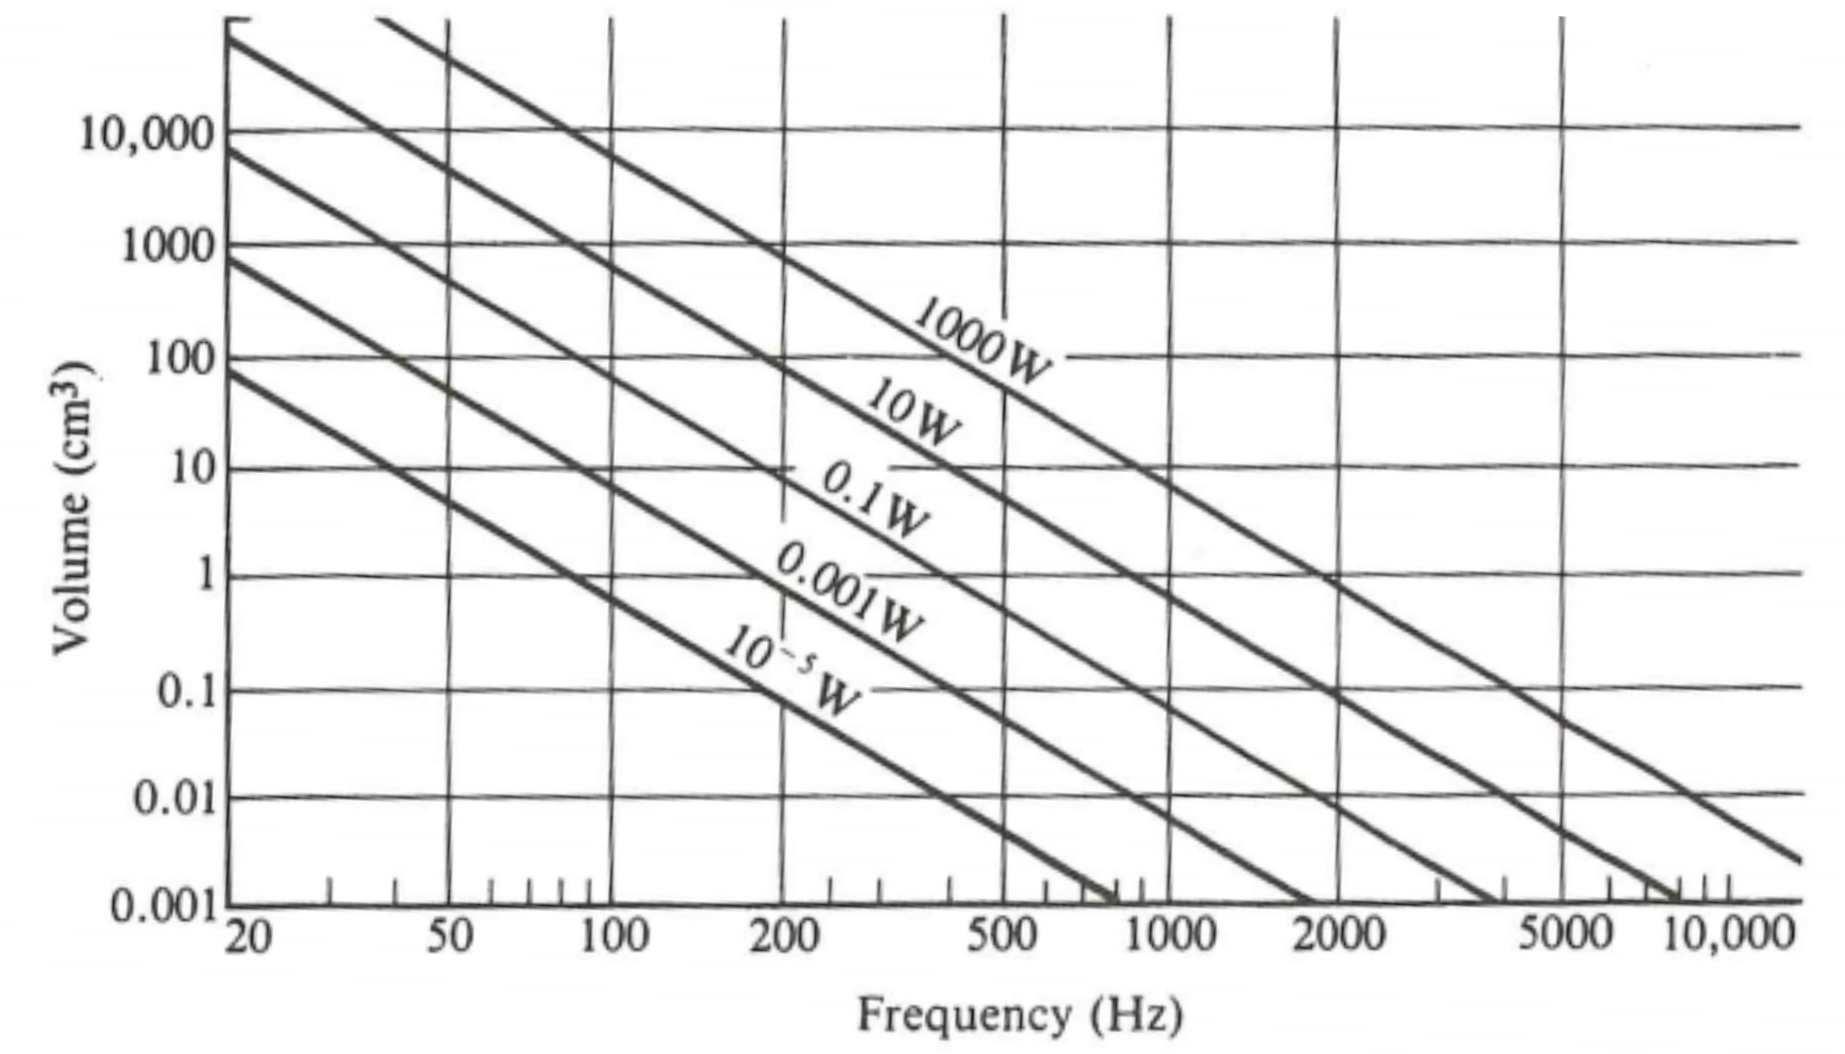
\includegraphics[scale=0.7]{figures/oving3_1.png}
    \caption{Volume of air moved by speaker as a function of sound power and frequency. Illustration from "Science of Sound", Chapter 23.}
    \label{fig:abs}
\end{figure}



\end{document}